\documentclass[tikz,border=0pt]{standalone}
\usepackage[american]{circuitikz}
\usetikzlibrary{arrows.meta,calc,positioning,decorations.pathmorphing,patterns}
\definecolor{zyloTeal}{HTML}{174A5B}
\definecolor{zyloTealTwo}{HTML}{246B7A}
\definecolor{zyloInk}{HTML}{1F2933}
\definecolor{zyloSoft}{HTML}{EAF4F4}
\definecolor{zyloPaper}{HTML}{F8FAFB}
\definecolor{zyloLine}{HTML}{44606B}
\definecolor{zyloOrange}{HTML}{D97706}
\begin{document}
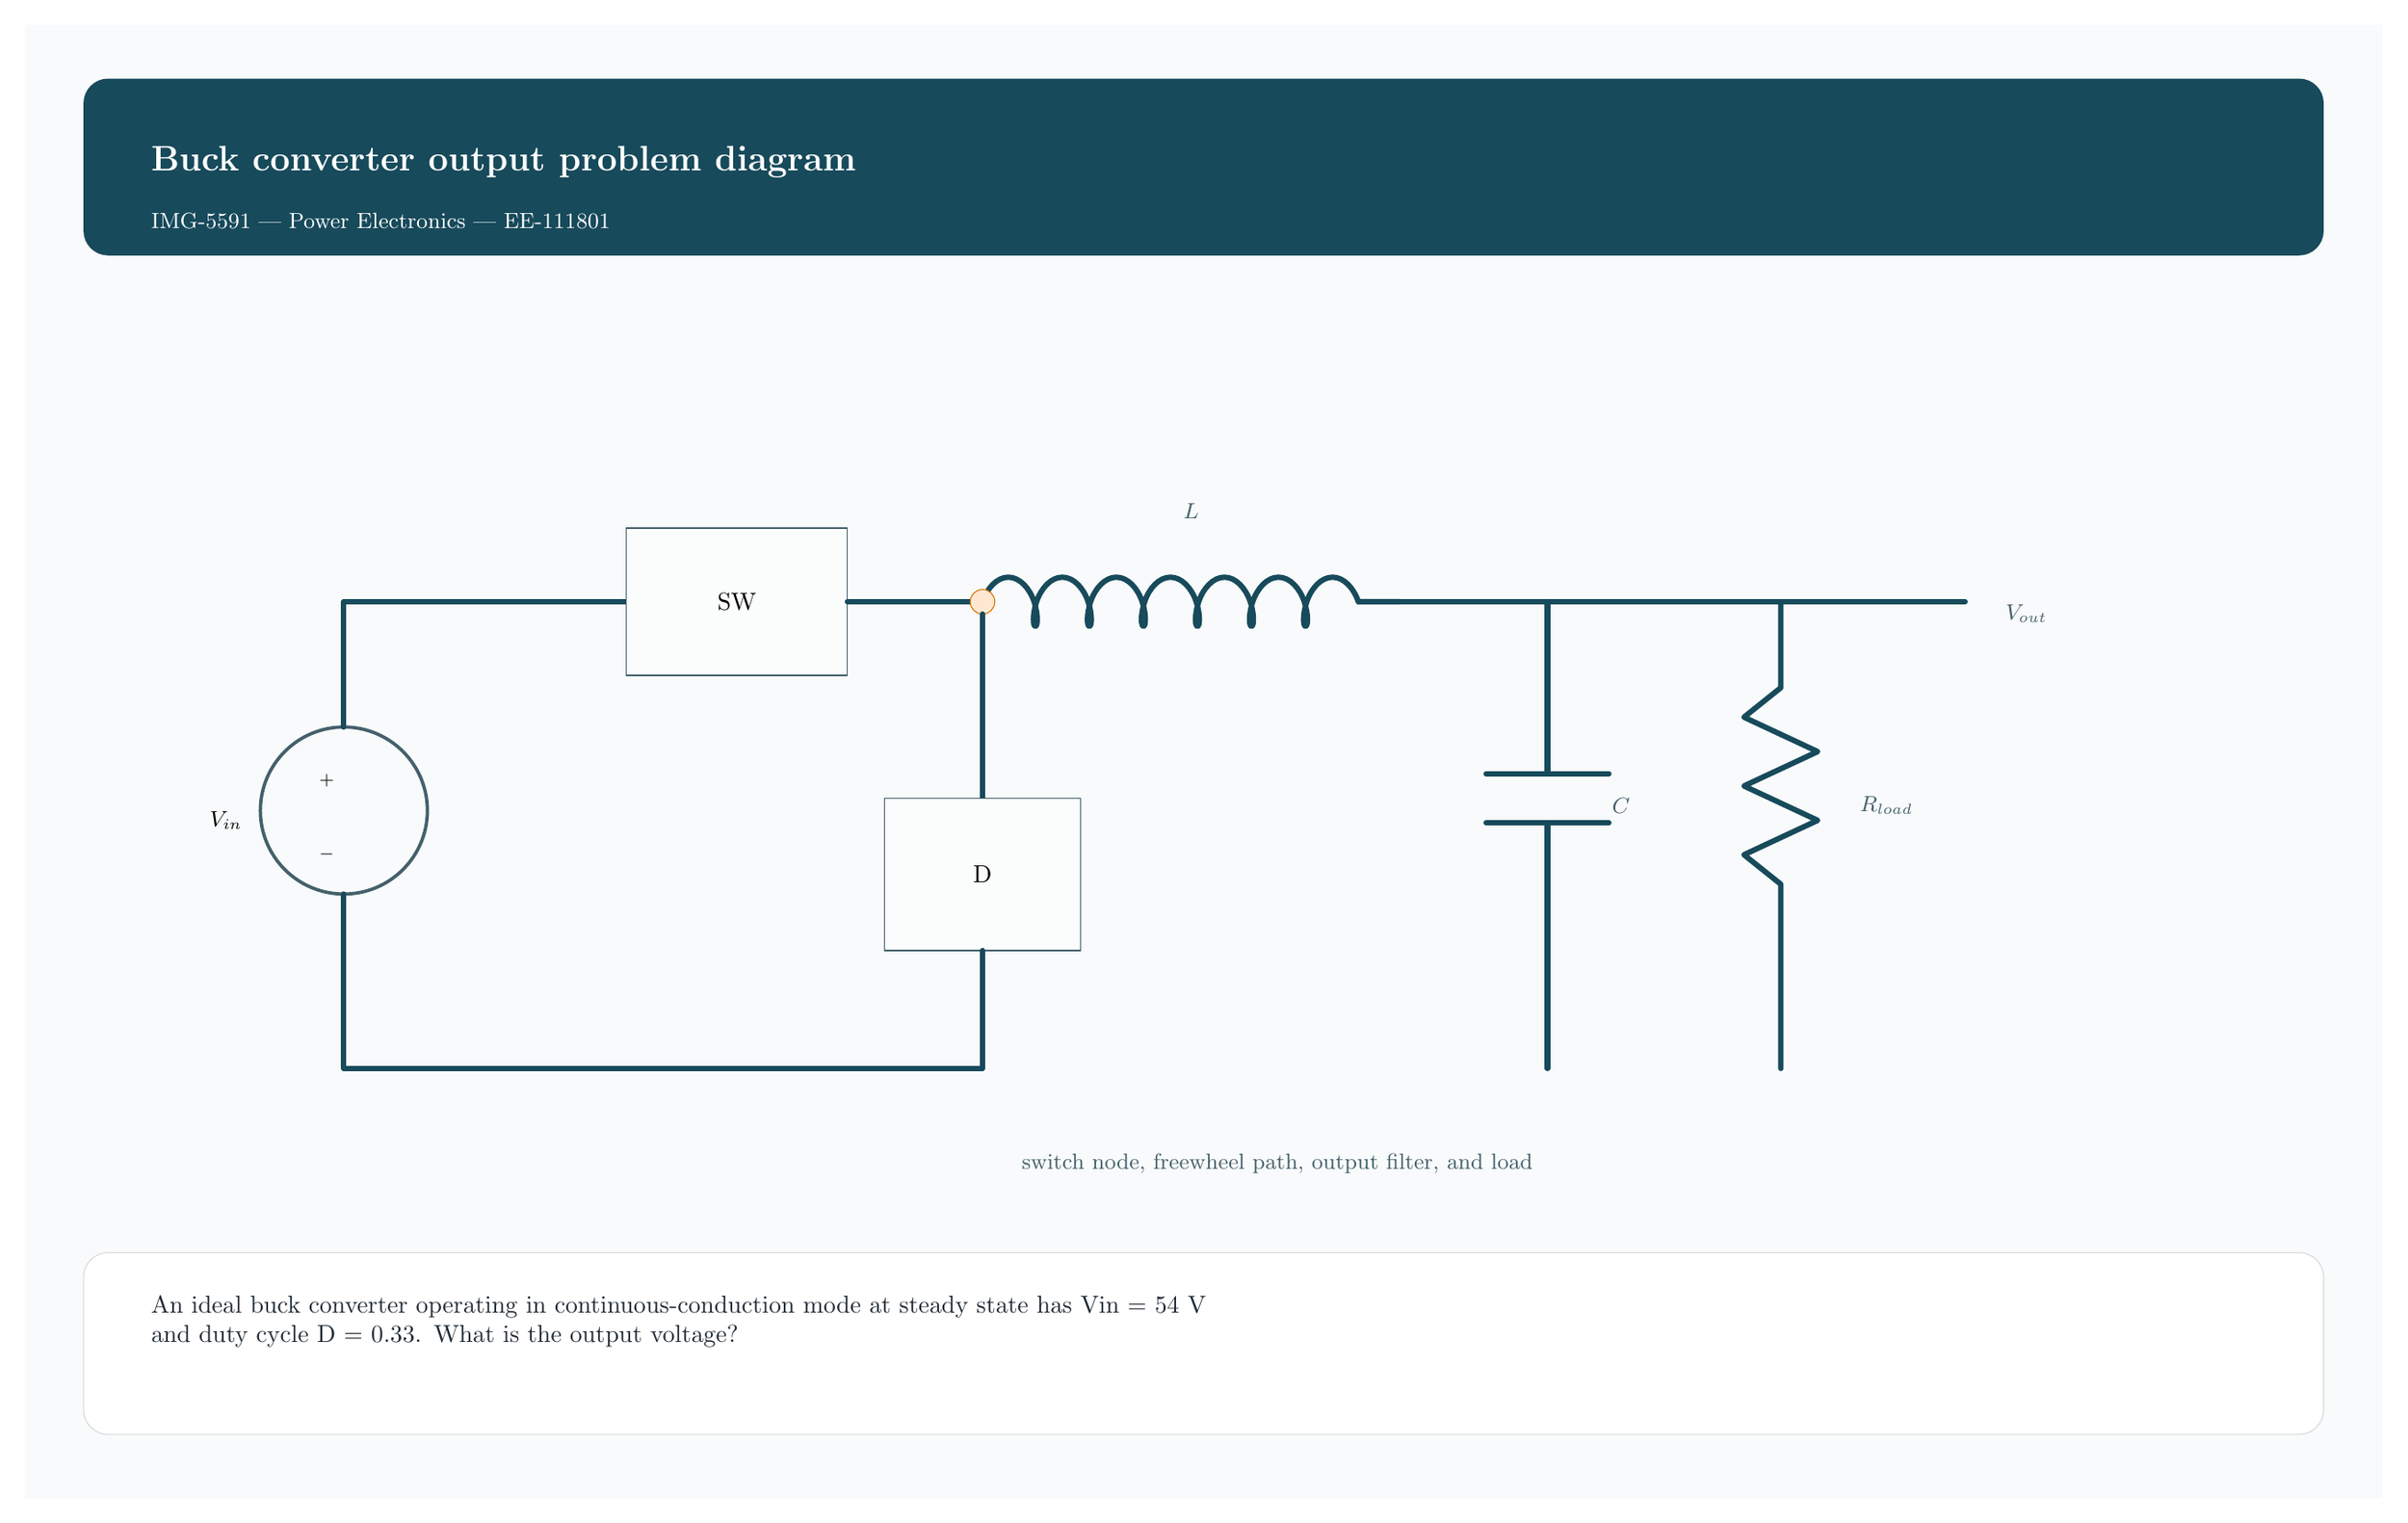
\begin{tikzpicture}[x=1pt,y=-1pt,>=Latex,line cap=round,line join=round]
\path[fill=zyloPaper] (0,0) rectangle (960,600);
\path[fill=zyloTeal,rounded corners=10pt] (24,22) rectangle (936,94);
\node[anchor=west,text=white,font=\bfseries\Large] at (48,56) {Buck converter output problem diagram};
\node[anchor=west,text=white!82,font=\small] at (48,80) {IMG-5591 | Power Electronics | EE-111801};
\tikzset{wire/.style={draw=zyloTeal,line width=2.2pt},thinwire/.style={draw=zyloLine,line width=1.35pt},accent/.style={draw=zyloOrange,line width=2.2pt},box/.style={draw=zyloTealTwo,fill=zyloSoft,line width=1.5pt,rounded corners=8pt}}
\draw[thinwire] (130,320) circle (34); \node[font=\scriptsize] at (123,308) {$+$}; \node[font=\scriptsize] at (123,338) {$-$}; \node[font=\small] at (82,324) {$V_{in}$};
\draw[wire] (130,286) -- (130,235) -- (245,235); \node[draw=zyloLine,fill=white!80!zyloSoft,minimum width=90pt,minimum height=60pt] at (290,235) {SW};
\draw[wire] (335,235) -- (390,235); \draw[wire,decorate,decoration={coil,aspect=0.5,segment length=22pt,amplitude=10pt}] (390,235) -- (560,235); \draw[wire] (560,235) -- (790,235);
\filldraw[draw=zyloOrange,fill=orange!18] (390,235) circle (5); \draw[wire] (390,240) -- (390,315); \node[draw=zyloLine,fill=white!80!zyloSoft,minimum width=80pt,minimum height=62pt] at (390,346) {D}; \draw[wire] (390,377) -- (390,425) -- (130,425) -- (130,354);
\draw[wire] (620,235) -- (620,305); \draw[wire] (595,305) -- (645,305); \draw[wire] (595,325) -- (645,325); \draw[wire] (620,325) -- (620,425);
\draw[wire] (715,235) -- (715,270) -- (700,282) -- (730,296) -- (700,310) -- (730,324) -- (700,338) -- (715,350) -- (715,425);
\node[font=\small,text=zyloLine] at (475,198) {$L$}; \node[font=\small,text=zyloLine] at (650,318) {$C$}; \node[font=\small,text=zyloLine] at (758,318) {$R_{load}$}; \node[font=\small,text=zyloLine] at (815,240) {$V_{out}$};
\node[font=\small,text=zyloLine] at (510,464) {switch node, freewheel path, output filter, and load};
\path[draw=black!15,fill=white,rounded corners=10pt] (24,500) rectangle (936,574);
\node[anchor=west,text width=860pt,align=left,text=zyloInk,font=\normalsize] at (48,528) {An ideal buck converter operating in continuous-conduction mode at steady state has Vin = 54 V\\and duty cycle D = 0.33. What is the output voltage?};
\end{tikzpicture}
\end{document}
